\section{The HEP community and LHC}
\begin{figure}
    \centering
    \subfloat[LHC accelerator]{
    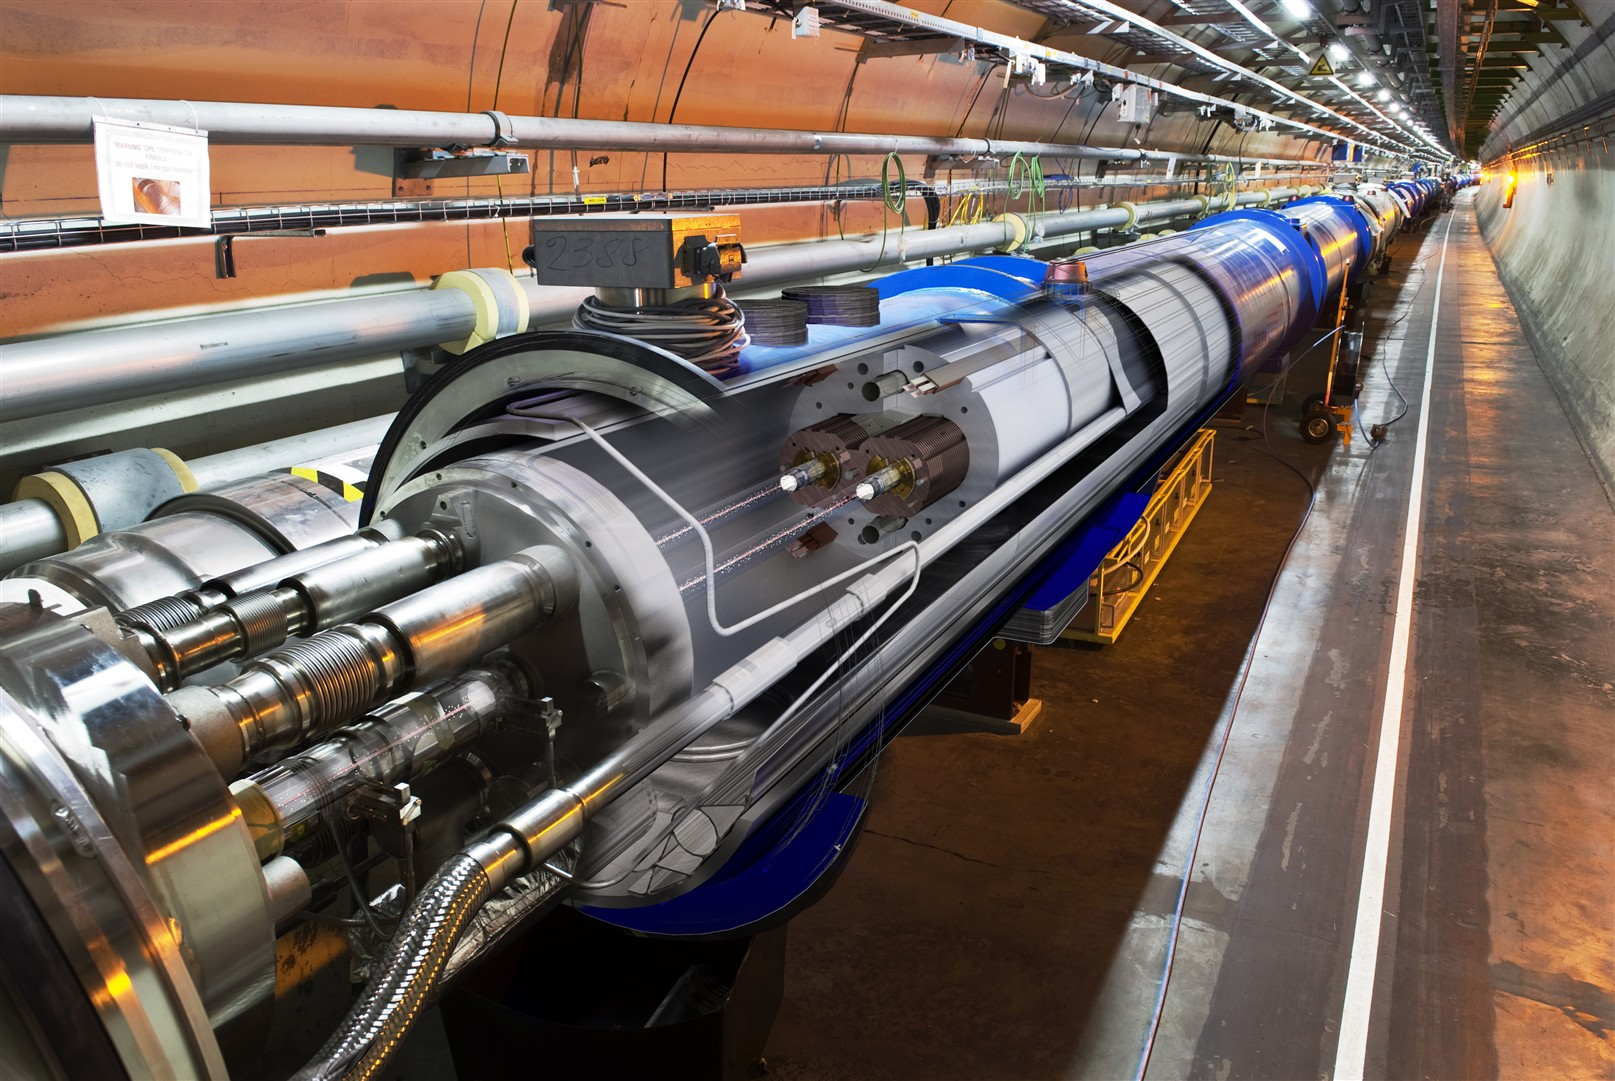
\includegraphics[width=\textwidth]{figures/220_introduction/cern/a0lhcinternotubo_445034351.jpg}\label{fig:lhc:pipes}
    }
    
    \subfloat[Aerial view]{
    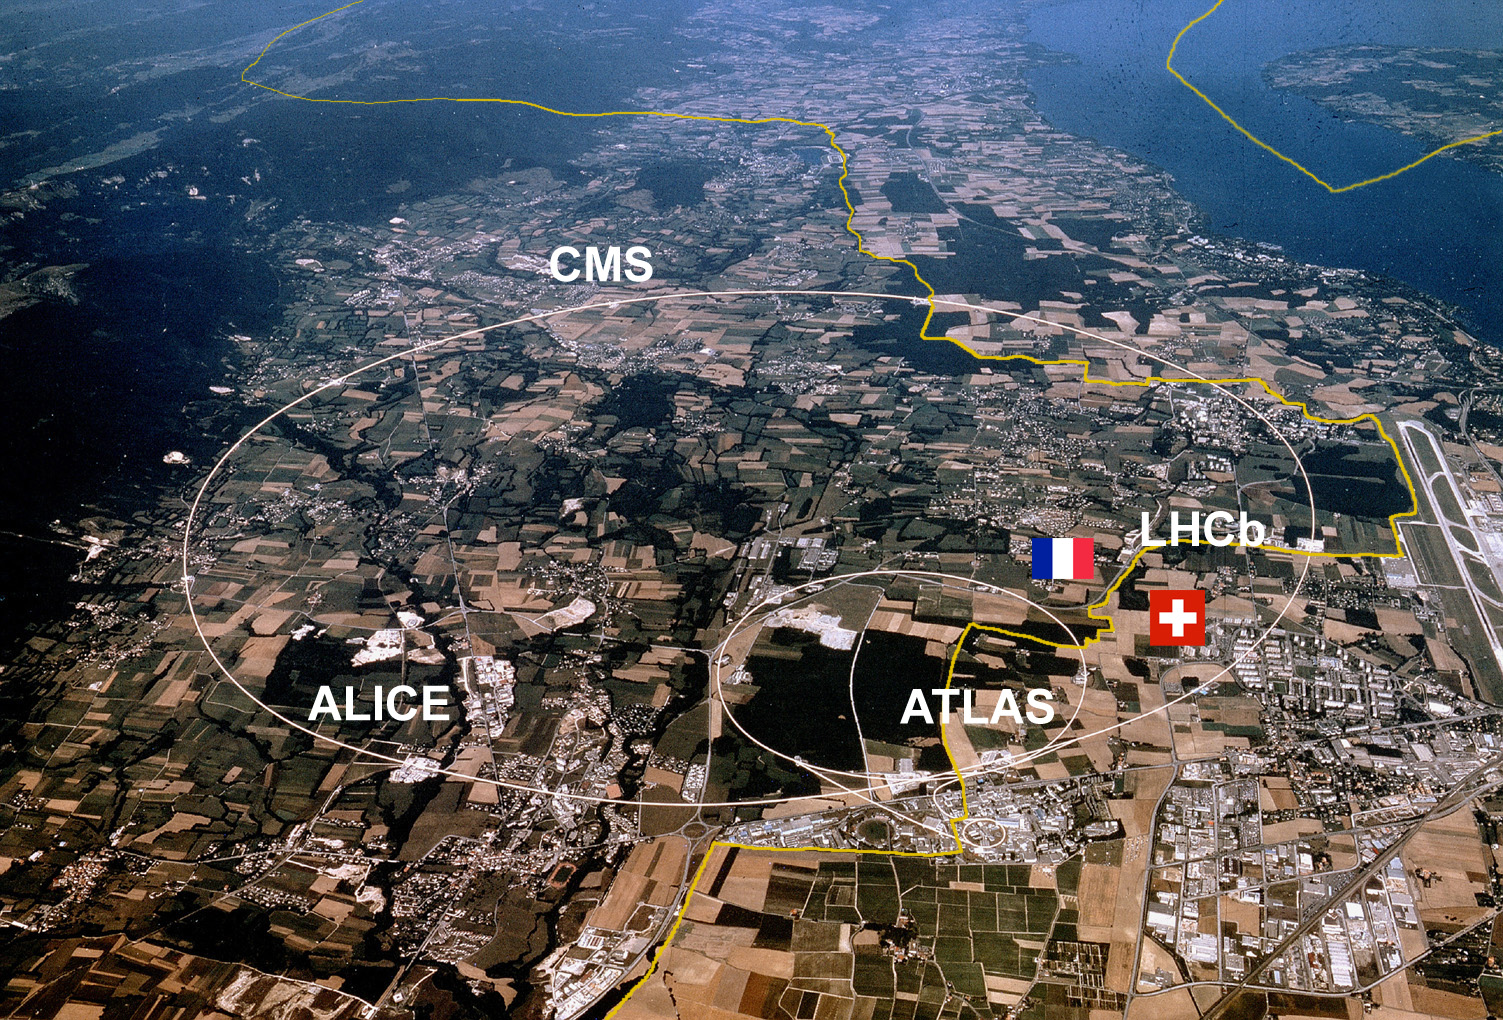
\includegraphics[width=0.5\textwidth]{figures/220_introduction/cern/CERN_location.jpg}\label{fig:lhc:location}
    }
    \subfloat[LHC scheme]{
    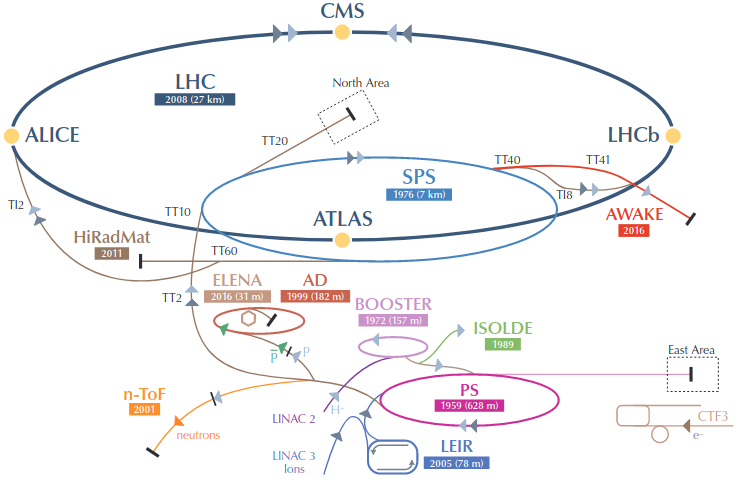
\includegraphics[width=0.5\textwidth]{figures/220_introduction/cern/lhc_scheme_factsfigures.png}\label{fig:lhc:schema}
    }
    \caption{\textbf{LHC accelerator complex.} (\hyperref[fig:lhc:pipes]{a}) the underground tunnel that hosts LHC and its transverse section;
    (\hyperref[fig:lhc:location]{b}) aerial view of the LHC complex at the boundary between Switzerland and France; (\hyperref[fig:lhc:schema]{c}) schema of the various LHC accelerating structures. The pictures are borrowed from various online sources: (\href{https://www.ansa.it/scienza/notizie/rubriche/fisica/2015/03/12/lacceleratore-lhc-pronto-a-ripartire-entro-2-settimane_60eed799-e47a-46e3-8908-056254a03a26.html?idPhoto=1}{1}), (\href{https://aec-analisiecalcolo.it/pubblicazioni/aec/86/656/}{2}), (\href{https://home.cern/science/accelerators/accelerator-complex}{3})
    }
    \label{fig:lhc}
\end{figure}

\begin{figure}
    \centering
    \subfloat[ALICE]{
    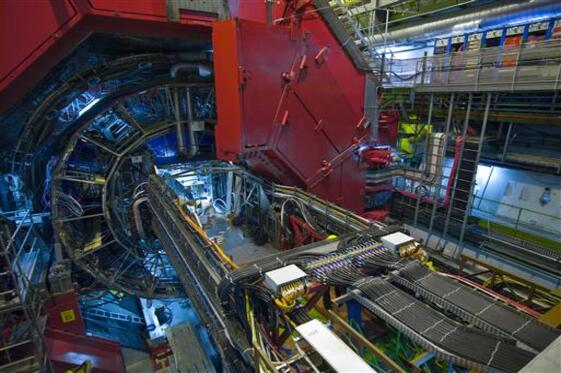
\includegraphics[width=0.5\textwidth]{figures/220_introduction/cern/alice_detector_medium1.jpg}
    }
    \subfloat[ATLAS]{
    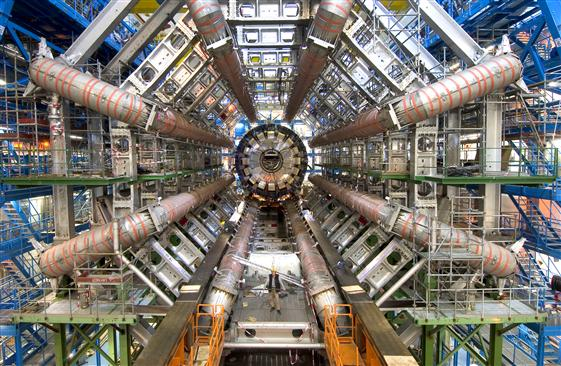
\includegraphics[width=0.5\textwidth]{figures/220_introduction/cern/atlas_detector_medium.jpg}
    }
    
    \subfloat[CMS]{
    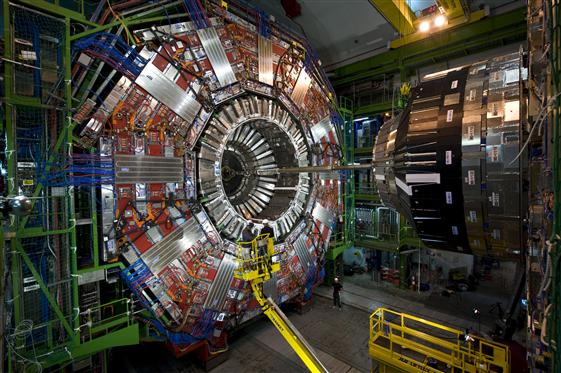
\includegraphics[width=0.5\textwidth]{figures/220_introduction/cern/cms_detector_medium1.jpg}
    }
    \subfloat[LHCb]{
    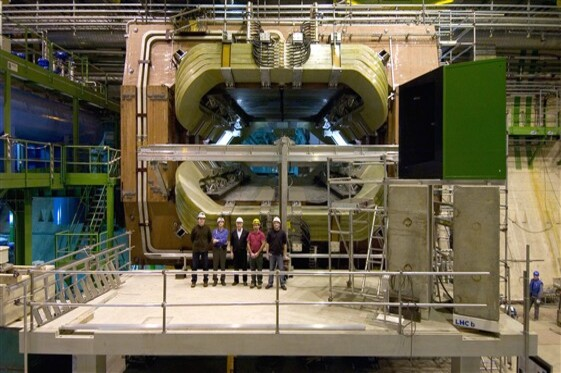
\includegraphics[width=0.5\textwidth]{figures/220_introduction/cern/lhcb_detector_medium.jpg}
    }
    \caption{\textbf{CERN major experiments.}
    The images are borrowed from the CERN experiments \href{https://home.cern/resources/image/experiments}{image gallery}
    }
    \label{fig:cern_experiments}
\end{figure}

% High-Energy Physics (HEP) is a branch of physics that studies the fundamental constituents of matter and the forces that drive their interactions. One of the methods is to create very high energy densities. 
% This reproduces the environmental conditions of the primordial universe.

High-Energy Physics (HEP) is a branch of physics that studies the elementary constituents of matter and the fundamental principles that govern their interaction to understand how our universe has formed and is evolving.  
These particles, however, are not visible at the scales whereby we experience reality today. 
Thus, HEP experiments need to either look at natural phenomena generated in pressure and temperature conditions similar to those of the primordial universe -- like cosmic rays -- or recreate such settings artificially.

The European Council for Nuclear Research (CERN) is part of this second strand of experiments, and it constitutes the largest particle physics laboratory in the world.
From 2008, CERN facilities also include the Large Hadron Collider (LHC), the longest particle accelerator ever built.
LHC consists of a \mbox{26.7-kilometer} ring located in a tunnel about 100 meters underground in the Geneva area (\cref{fig:lhc}), and it is made of superconducting magnets with several accelerating structures \cite{lhcwebsite}.
Inside the accelerator, bunches of protons are revved up to nearly the speed of light, forming two high-energy particle beams that travel in opposite directions inside separated pipes. 
When they acquire the desired energy, the beams are directed towards dedicated interaction points where the experiments occur. %surrounded by giant detectors.
In practice, LHC hosts four major experiments built in correspondence of these locations -- ALICE \cite{aamodt2008alice}, ATLAS \cite{aad2008atlas}, CMS \cite{collaboration2008cms} and LHCb \cite{alves2008lhcb} -- and equipped with giant detectors (\cref{fig:cern_experiments}).
Once the beams get there, the two pipes cross and the particles are squeezed through substantial magnetic fields to increase their chances of colliding. 
In this way, a massive amount of energy is concentrated in an extremely tiny area, generating billions of particles at each collision.
Indeed, the high intensity of the beams causes roughly 40 million crossings per second at each interaction point \cite{albrecht2019roadmap, grandi2017HEPsize}. 
When a crossing happens, an average of 60 bunch collisions -- also referred to as pileup -- are observed \cite{albrecht2019roadmap}. The particles produced by each scattering then fly around the interaction point to be eventually detected through high-technology experimental devices endowed with over 100 million electronic channels \cite{grandi2017HEPsize, aad2020channels}.
According to the latest experimental setup, this delivers 100 MegaBytes (MB) of data per collision and it would generate 40k ExaBytes (EB) every year \cite{grandi2017HEPsize}.
However, storing such a tremendous amount of data is unattainable with current technology and budget. In addition, the events of interest are typically rare, so there is actually no need to record all of the information detected by the electronic channels.
Thus, the vast majority of \emph{read-out} data from collisions is discarded straight away using hardware and software trigger selection systems, thus lowering the \emph{recorded} event rate to 1k crossings per second. 
As a result of this reduction, the actual acquisition rate
% amounts to 1MB every second, translating to roughly 100 PetaBytes (PB) a year in 2018 \cite{grandi2017HEPsize, altre?}.
amounts to nearly 1 PetaBytes (PB) per day \cite{cern2017storage}, translating to roughly 160 PB%
\footnote{LHC registered 161 days of physics data taking in 2018 \cite{todd2018lhcAvail}}
a year in 2018. %\cite{grandi2017HEPsize, cern2017datayear}.
Besides that, physics analyses require comparing experimental results with Monte Carlo data simulated according to current theories, thus producing somewhat between 1 and 2 times additional data \cite{grandi2017HEPsize}.
Furthermore, the CERN community is already working at enhancing the Large Hadron Collider capabilities.
The project involves boosting the energy of the beam and gradually increasing the pileup towards 200 collisions per bunch crossing \cite{albrecht2019roadmap}, thus leading to the so-called High Luminosity LHC (HL-LHC) \cite{hllhc}.
% Thanks to this upgrade, way more events will be observed as the beam energy will be boosted and the pileup will gradually be increased towards 150 collisions per bunch crossing.
% In this new regime, 
Thanks to this upgrade, the observed events are expected to increase of a factor $\geq5$ \cite{hllhc} and produce an estimated 800 PB of new data each year by 2026.%\cite{grandi2017HEPsize, HLLHC_data}.

Although it is difficult to replicate such a punctual measurement of the data production for other big data players, some hints can be retrieved by comparing multiple online resources \cite{clissa2022survey}. %\cite{BDPlot_series}. 
\Cref{fig:bigdata_size} tries to summarize a reasonable, up-to-date ``guesstimate"%
\footnote{These data are reconstructed based on multiple online sources about the amount of contents produced, streamed or hosted by big data companies and reasonable estimates of unitary sizes for such contents, e.g. average mail or picture size, average data traffic for 1 hour video, and so on. 
However, the actual values reported are not meant to be extremely accurate and only serve the purpose of giving an idea of the orders of magnitude of the various phenomena.
}
of yearly data production for the main big data companies.
Despite not being the most popular among the mainstream audience, the HEP community is one of the most prominent players concerning big data.
% \begin{landscape}
% \begin{figure}
%     \centering
% \begin{tikzpicture}%[shorten >=1pt,node distance=1cm,on grid,auto] 
% \linespread{.5}%
% \begin{scope}
%     \node[anchor=south west,inner sep=0] (image) at (0,0){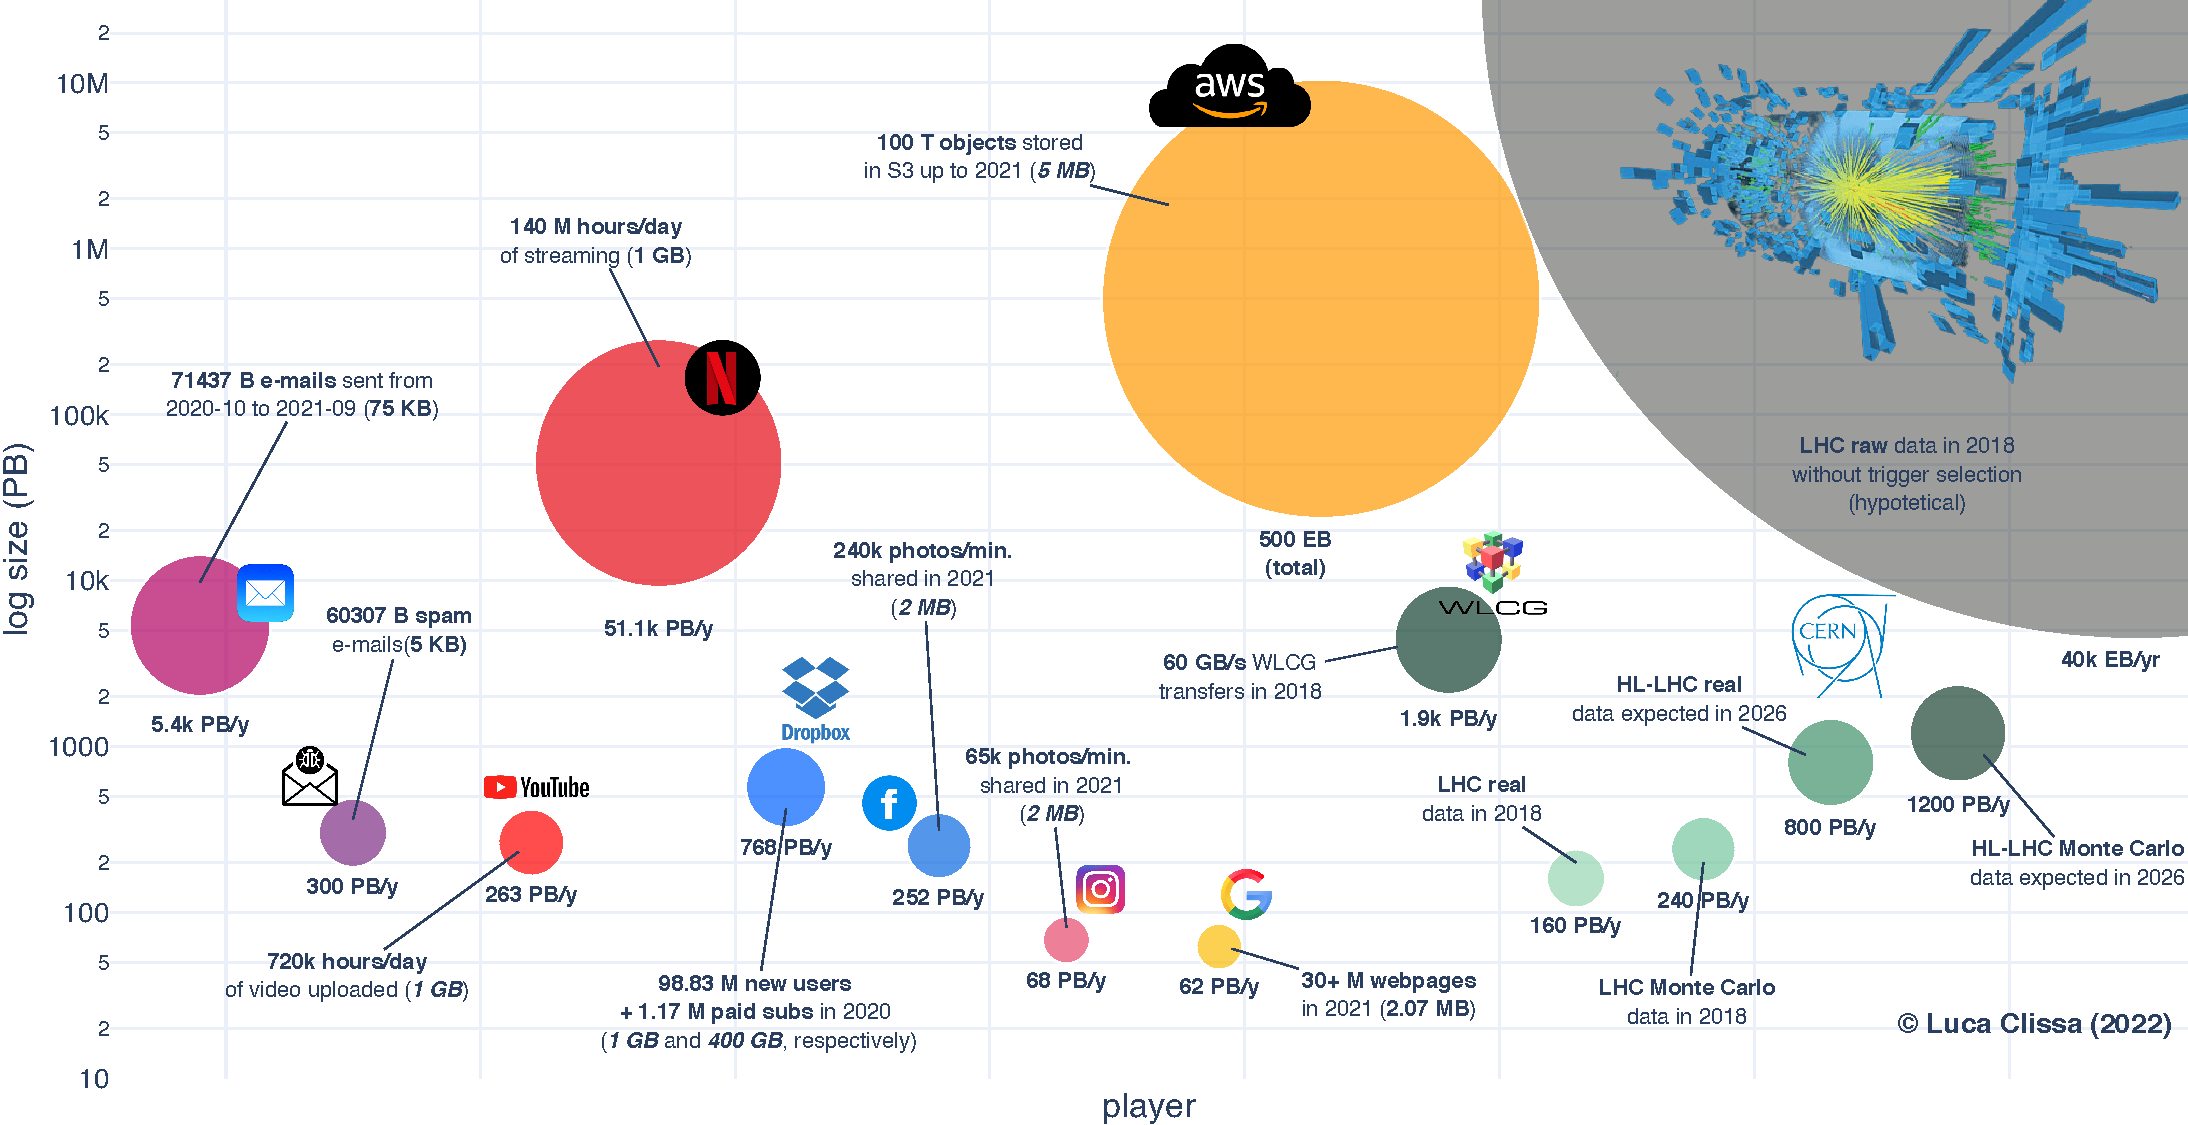
\includegraphics[width=\linewidth]{figures/220_introduction/BigData2021.pdf}};
% \begin{scope}[x={(image.south east)},y={(image.north west)}]
%     \node [anchor=west] (note1) at (0.26,0.170) {\href{https://stackoverflow.com}{Link}};
%         \node [anchor=west, scale=1, align=center,font=\tiny] (note2) at (0.26,0.470) {\href{https://rdcu.be/cB1Ds}{paper} \\ from the future};
% \end{scope}
%     \end{scope}
% \end{tikzpicture}
% \caption{\textbf{Big Data sizes.} Bubble plot of the orders of magnitude of data produced by important big data players. The balloon areas illustrate the amount of data and the text annotations highlight the key factors considered in the estimates. Average per-unit-sizes are reported in parentheses, where italic indicates measures reconstructed based on likely assumptions because no references were found.} \label{fig:bigdata_size1}
% \end{figure}
% \end{landscape}
\begin{landscape}
\begin{figure}
    \centering
    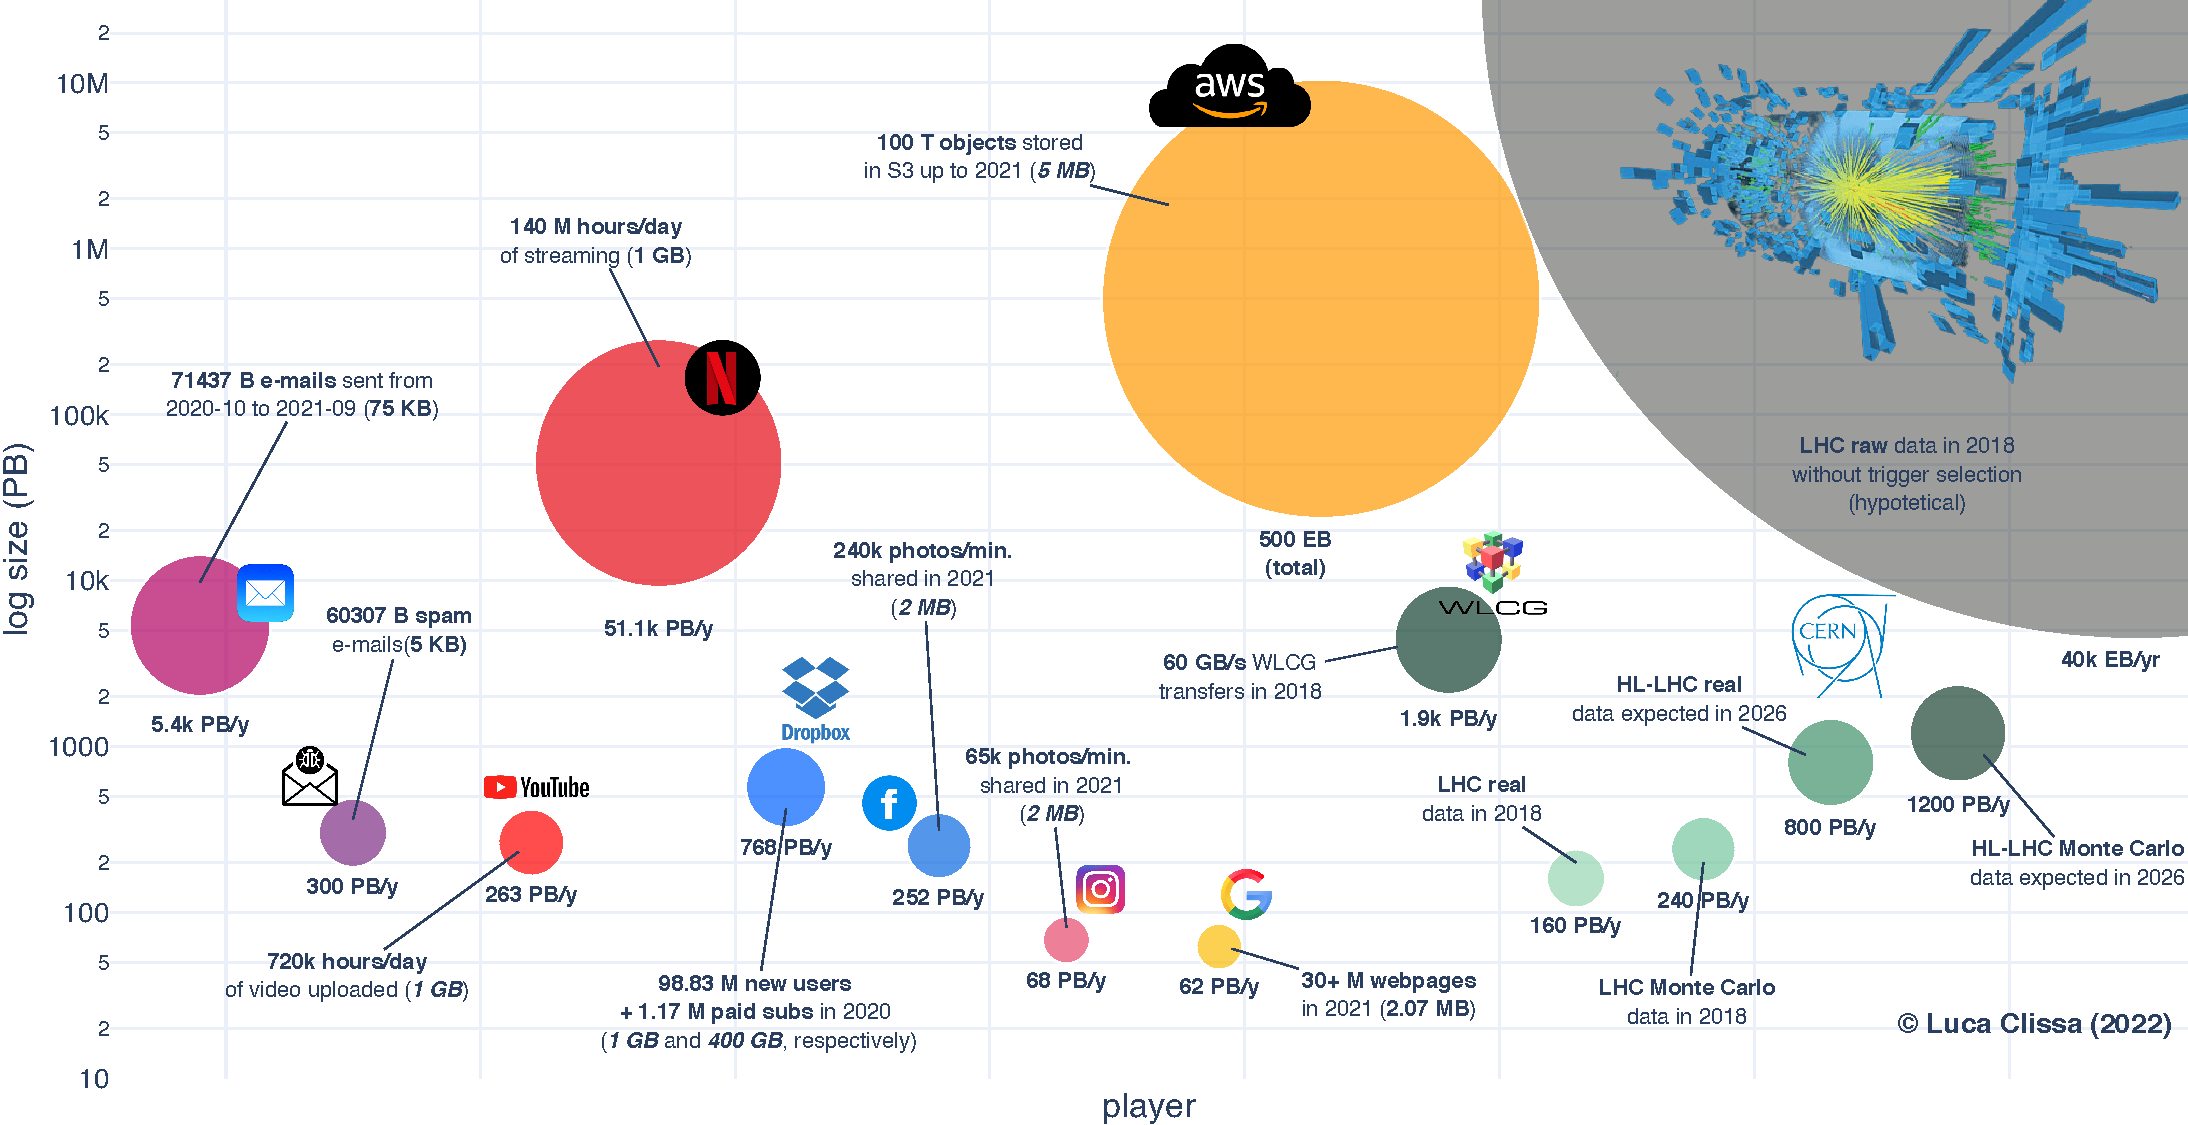
\includegraphics[width=\linewidth]{figures/220_introduction/BigData2021.pdf}
    \caption{\textbf{Big Data sizes.} Bubble plot of the orders of magnitude of data produced by important big data players. The balloon areas illustrate the amount of data and the text annotations highlight the key factors considered in the estimates. Average per-unit sizes are reported in parentheses, where italic indicates measures reconstructed based on likely assumptions because no references were found. Interactive version available at: \href{https://clissa.github.io/BigData2021/BigData2021.html}{BigData2021.html}}
    \label{fig:bigdata_size}
\end{figure}
\end{landscape}

Indeed the read-out data LHC produced every year in Phase 2 (40k EB) is around one order of magnitude bigger than the total size of objects ever stored on Amazon AWS cloud service (500 EB)%
\footnote{Obtained considering the total number of objects reportedly stored in Amazon S3 (100 trillion, \citeA{amazon2021objectscount}) and assuming an average size of 5 MB based on some average bucket example \cite{amazon2021objectssize}}.
Considering effectively recorded data, LHC figures are comparable with those of other most renowned big data entities. The last run (2018), in fact, produced hundreds of PetaBytes (PB) (roughly 160 of real data and 240 of Monte Carlo simulations),
 which is similar to the orders of magnitude generated by Google searches (62 PB)%
\footnote{Obtained considering that Google search index contains at least 30 billion web pages \cite{van2016estimating, google2021index_size, djuraskovic2020googl_stats, indig2020index_size} and that the average page size is 2.15 MB \cite{http2021webpage_size}
},
Instagram and Facebook shared photos (68 and 252 PB, respectively)%
\footnote{Obtained considering that 65k and 240k pictures are shared every minute on Instagram and Facebook \cite{domo2021infographic}, and assuming 2 MB as a reasonable average picture size \cite{adobe2021fb_img_size}
}
and YouTube video uploads (263 PB)%
\footnote{Obtained considering that 720k hours of video are uploaded daily \cite{dean2021youtube} and assuming an average size of 1 GB \cite{quora2021youtube}
}.
Moreover, LHC will climb the table even further with the upgrade to high luminosity, when the real and Monte Carlo data production rate is expected to rise to levels comparable to those of storage services like Dropbox (800, 1200 and 768 PB%
\footnote{Obtained considering that Dropbox registered 100 million of new users in 2020, 1.17 million of which were paid subscriptions \cite{dean2021dropbox}. For the average per-unit size, it was assumed that free accounts exploited 75\% of the 2 GB storage available, while paid ones exploited 25\% of the total 2 TB
}, respectively). 

Apart from the nominal values of the generated information, streaming data comprise a significant slice of the big data market.
As a matter of fact, the continual movement of small- to medium-sized files spawns massive traffic when scaled up to millions of users, as testified by e-mails (5.7k PB)%
\footnote{Obtained considering that 71k billion e-mails and 60k billion spam messages were sent from October 2020 to September 2021 \cite{statista2021mails}, and that the average size is \mbox{75 KB} for e-mails \cite{lifewire2021avg_mail} and \mbox{5} KB for spam \cite{medium2014avg_spam}
},
and Netflix (51.1k PB)%
\footnote{Obtained considering that Netflix users consumed 140 million hours per day of streaming \cite{domo2021infographic} and that counts for 1 GB of data for standard definition videos \cite{perry2021netflix}
} bubbles in \cref{fig:bigdata_size}.
% Also in this respect, LHC plays an important role. Indeed, the HEP community is formed by thousands of researchers spread around the world that need to access the data produced at CERN.
A similar usage is generated also by the LHC, whose data are continuously transferred across the HEP community thanks to the Worldwide LHC Computing Grid (see \cref{wlcg}) to fuel innovative research. For example, 
% 12 PB of data were accessed on average every day in 2020 for the ATLAS experiment alone \cite{calafiura2020design_report}, and
a throughput of 60 GB/s was generated by the 4 experiments together in 2018 \cite{wlcg2018throughput} thus giving a yearly projection (1.9k PB) close to half of the global e-mails traffic and only one order of magnitude lower than Netflix usage.
% Indeed, thousands of researchers from all around the world need to access LHC data, analyze them and share their results to investigate new theories and advance our knowledge of the universe.
% For this reason, the Worldwide LHC Computing Grid computing infrastructure has been developed over the years 

Given the large quantities of data involved by the LHC, it is not surprising how careful planning must be done in order to meet the needs of the LHC community, and tailored strategies and technologies must be adopted to cope with such requirements. 
Luckily, the presence of other stakeholders facing analogous problems provides the HEP community with some alternatives to draw from, and it allows researchers to tap in from existing solutions and customize them for their necessities.